% Options for packages loaded elsewhere
\PassOptionsToPackage{unicode}{hyperref}
\PassOptionsToPackage{hyphens}{url}
\PassOptionsToPackage{dvipsnames,svgnames,x11names}{xcolor}
%
\documentclass[
  letterpaper,
  DIV=11,
  numbers=noendperiod]{scrartcl}

\usepackage{amsmath,amssymb}
\usepackage{iftex}
\ifPDFTeX
  \usepackage[T1]{fontenc}
  \usepackage[utf8]{inputenc}
  \usepackage{textcomp} % provide euro and other symbols
\else % if luatex or xetex
  \usepackage{unicode-math}
  \defaultfontfeatures{Scale=MatchLowercase}
  \defaultfontfeatures[\rmfamily]{Ligatures=TeX,Scale=1}
\fi
\usepackage{lmodern}
\ifPDFTeX\else  
    % xetex/luatex font selection
\fi
% Use upquote if available, for straight quotes in verbatim environments
\IfFileExists{upquote.sty}{\usepackage{upquote}}{}
\IfFileExists{microtype.sty}{% use microtype if available
  \usepackage[]{microtype}
  \UseMicrotypeSet[protrusion]{basicmath} % disable protrusion for tt fonts
}{}
\makeatletter
\@ifundefined{KOMAClassName}{% if non-KOMA class
  \IfFileExists{parskip.sty}{%
    \usepackage{parskip}
  }{% else
    \setlength{\parindent}{0pt}
    \setlength{\parskip}{6pt plus 2pt minus 1pt}}
}{% if KOMA class
  \KOMAoptions{parskip=half}}
\makeatother
\usepackage{xcolor}
\setlength{\emergencystretch}{3em} % prevent overfull lines
\setcounter{secnumdepth}{5}
% Make \paragraph and \subparagraph free-standing
\ifx\paragraph\undefined\else
  \let\oldparagraph\paragraph
  \renewcommand{\paragraph}[1]{\oldparagraph{#1}\mbox{}}
\fi
\ifx\subparagraph\undefined\else
  \let\oldsubparagraph\subparagraph
  \renewcommand{\subparagraph}[1]{\oldsubparagraph{#1}\mbox{}}
\fi


\providecommand{\tightlist}{%
  \setlength{\itemsep}{0pt}\setlength{\parskip}{0pt}}\usepackage{longtable,booktabs,array}
\usepackage{calc} % for calculating minipage widths
% Correct order of tables after \paragraph or \subparagraph
\usepackage{etoolbox}
\makeatletter
\patchcmd\longtable{\par}{\if@noskipsec\mbox{}\fi\par}{}{}
\makeatother
% Allow footnotes in longtable head/foot
\IfFileExists{footnotehyper.sty}{\usepackage{footnotehyper}}{\usepackage{footnote}}
\makesavenoteenv{longtable}
\usepackage{graphicx}
\makeatletter
\def\maxwidth{\ifdim\Gin@nat@width>\linewidth\linewidth\else\Gin@nat@width\fi}
\def\maxheight{\ifdim\Gin@nat@height>\textheight\textheight\else\Gin@nat@height\fi}
\makeatother
% Scale images if necessary, so that they will not overflow the page
% margins by default, and it is still possible to overwrite the defaults
% using explicit options in \includegraphics[width, height, ...]{}
\setkeys{Gin}{width=\maxwidth,height=\maxheight,keepaspectratio}
% Set default figure placement to htbp
\makeatletter
\def\fps@figure{htbp}
\makeatother

% load packages
\usepackage{geometry}
\usepackage{xcolor}
\usepackage{eso-pic}
\usepackage{fancyhdr}
\usepackage{sectsty}
\usepackage{fontspec}
\usepackage{titlesec}

%% Set page size with a wider right margin
\geometry{a4paper, total={170mm,257mm}, left=20mm, top=20mm, bottom=20mm, right=50mm}

%% Let's define some colours
\definecolor{uniblue}{HTML}{003865}
\definecolor{burgundy}{HTML}{7D2239}
\definecolor{cobalt}{HTML}{005C8A}
\definecolor{lavender}{HTML}{5B4D94}
\definecolor{leaf}{HTML}{006630}
\definecolor{moss}{HTML}{385A4F}
\definecolor{pillarbox}{HTML}{B30C00}
\definecolor{rust}{HTML}{9A3A06}
\definecolor{sandstone}{HTML}{52473B}
\definecolor{skyblue}{HTML}{005398}
\definecolor{slate}{HTML}{4F5961}
\definecolor{thistle}{HTML}{951272}

%\definecolor{light}{HTML}{E6E6FA} % original from template - redefined below as uni blue at 10 percent:
\colorlet{light}{uniblue!10}
%\definecolor{highlight}{HTML}{800080} % original from template - redefined below as uni's skyblue:
\colorlet{highlight}{skyblue}
%\definecolor{dark}{HTML}{330033} % original from template - redefined below as uni blue at 100 percent:
\colorlet{dark}{uniblue}

%% Let's add the border on the right hand side 
\AddToShipoutPicture{% 
    \AtPageLowerLeft{% 
        \put(\LenToUnit{\dimexpr\paperwidth-3cm},0){% 
            \color{light}\rule{3cm}{\LenToUnit\paperheight}%
          }%
     }%
     % logo
    \AtPageLowerLeft{% start the bar at the bottom right of the page
        \put(\LenToUnit{\dimexpr\paperwidth-2.25cm},27.2cm){% move it to the top right
            \color{light}
\includegraphics[width=2.25cm]{_extensions/nrennie/PrettyPDF/uni_logo_boxed.jpg}
          }%
     }%
}

%% Style the page number
\fancypagestyle{mystyle}{
  \fancyhf{}
  \renewcommand\headrulewidth{0pt}
  \fancyfoot[R]{\thepage}
  \fancyfootoffset{3.5cm}
}
\setlength{\footskip}{20pt}

%% style the chapter/section fonts
\chapterfont{\color{uniblue}\fontsize{20}{16.8}\selectfont}
\sectionfont{\color{uniblue}\fontsize{20}{16.8}\selectfont}
\subsectionfont{\color{skyblue}\fontsize{14}{16.8}\selectfont}
\titleformat{\subsection}
  {\color{uniblue!90}\sffamily\Large\bfseries}{\thesubsection}{1em}{}[{\titlerule[0.8pt]}]
\subsubsectionfont{\color{cobalt}}

\renewcommand\thesection{\color{slate}\arabic{section}}
  
% left align title
\makeatletter
\renewcommand{\maketitle}{\bgroup\setlength{\parindent}{0pt}
\begin{flushleft}
  {\color{uniblue}\sffamily\huge\textbf{\@title}} \vspace{0.3cm} \newline
  {\Large {\@subtitle}} \newline
  \@author
\end{flushleft}\egroup
}
\makeatother

%% Use some custom fonts
\setsansfont{Ubuntu}[
    Path=_extensions/nrennie/PrettyPDF/Ubuntu/,
    Scale=0.9,
    Extension = .ttf,
    UprightFont=*-Regular,
    BoldFont=*-Bold,
    ItalicFont=*-Italic,
    ]

\setmainfont{Ubuntu}[
    Path=_extensions/nrennie/PrettyPDF/Ubuntu/,
    Scale=0.9,
    Extension = .ttf,
    UprightFont=*-Regular,
    BoldFont=*-Bold,
    ItalicFont=*-Italic,
    ]
\KOMAoption{captions}{tableheading}
\makeatletter
\@ifpackageloaded{tcolorbox}{}{\usepackage[skins,breakable]{tcolorbox}}
\@ifpackageloaded{fontawesome5}{}{\usepackage{fontawesome5}}
\definecolor{quarto-callout-color}{HTML}{909090}
\definecolor{quarto-callout-note-color}{HTML}{0758E5}
\definecolor{quarto-callout-important-color}{HTML}{CC1914}
\definecolor{quarto-callout-warning-color}{HTML}{EB9113}
\definecolor{quarto-callout-tip-color}{HTML}{00A047}
\definecolor{quarto-callout-caution-color}{HTML}{FC5300}
\definecolor{quarto-callout-color-frame}{HTML}{acacac}
\definecolor{quarto-callout-note-color-frame}{HTML}{4582ec}
\definecolor{quarto-callout-important-color-frame}{HTML}{d9534f}
\definecolor{quarto-callout-warning-color-frame}{HTML}{f0ad4e}
\definecolor{quarto-callout-tip-color-frame}{HTML}{02b875}
\definecolor{quarto-callout-caution-color-frame}{HTML}{fd7e14}
\makeatother
\makeatletter
\@ifpackageloaded{caption}{}{\usepackage{caption}}
\AtBeginDocument{%
\ifdefined\contentsname
  \renewcommand*\contentsname{Table of contents}
\else
  \newcommand\contentsname{Table of contents}
\fi
\ifdefined\listfigurename
  \renewcommand*\listfigurename{List of Figures}
\else
  \newcommand\listfigurename{List of Figures}
\fi
\ifdefined\listtablename
  \renewcommand*\listtablename{List of Tables}
\else
  \newcommand\listtablename{List of Tables}
\fi
\ifdefined\figurename
  \renewcommand*\figurename{Figure}
\else
  \newcommand\figurename{Figure}
\fi
\ifdefined\tablename
  \renewcommand*\tablename{Table}
\else
  \newcommand\tablename{Table}
\fi
}
\@ifpackageloaded{float}{}{\usepackage{float}}
\floatstyle{ruled}
\@ifundefined{c@chapter}{\newfloat{codelisting}{h}{lop}}{\newfloat{codelisting}{h}{lop}[chapter]}
\floatname{codelisting}{Listing}
\newcommand*\listoflistings{\listof{codelisting}{List of Listings}}
\makeatother
\makeatletter
\makeatother
\makeatletter
\@ifpackageloaded{caption}{}{\usepackage{caption}}
\@ifpackageloaded{subcaption}{}{\usepackage{subcaption}}
\makeatother
\makeatletter
\@ifpackageloaded{tcolorbox}{}{\usepackage[skins,breakable]{tcolorbox}}
\makeatother
\makeatletter
\@ifundefined{shadecolor}{\definecolor{shadecolor}{rgb}{.97, .97, .97}}{}
\makeatother
\makeatletter
\@ifundefined{codebgcolor}{\definecolor{codebgcolor}{named}{light}}{}
\makeatother
\makeatletter
\ifdefined\Shaded\renewenvironment{Shaded}{\begin{tcolorbox}[breakable, frame hidden, boxrule=0pt, colback={codebgcolor}, enhanced, sharp corners]}{\end{tcolorbox}}\fi
\makeatother
\ifLuaTeX
  \usepackage{selnolig}  % disable illegal ligatures
\fi
\usepackage{bookmark}

\IfFileExists{xurl.sty}{\usepackage{xurl}}{} % add URL line breaks if available
\urlstyle{same} % disable monospaced font for URLs
\hypersetup{
  pdftitle={Introduction to Environmental and Ecological Statistics},
  colorlinks=true,
  linkcolor={highlight},
  filecolor={Maroon},
  citecolor={Blue},
  urlcolor={highlight},
  pdfcreator={LaTeX via pandoc}}

\title{Introduction to Environmental and Ecological Statistics}
\author{}
\date{}

\begin{document}
\maketitle

\pagestyle{mystyle}

\textbf{Environmental and Ecological Statistics} is an incredibly broad
term covering any form of statistics applied to environmental and
ecological issues. Key themes include climate change, environmental
regulation (e.g.~water and air quality) and biodiversity monitoring.
This course focuses on this theme rather than a particular type of
statistical methodology. We will look at a variety of statistical
methods, some of which you will know, and some which will be new.

The environment is (sometimes literally) a burning issue in the 21st
century. This brings increased focus and interest in statistics as a
subject, and how we are working to handle topics like climate change.
Below, we see some examples of how climate change reporting can be
presented.

\begin{tcolorbox}[enhanced jigsaw, breakable, bottomrule=.15mm, toprule=.15mm, colbacktitle=quarto-callout-note-color!10!white, bottomtitle=1mm, arc=.35mm, opacitybacktitle=0.6, titlerule=0mm, colframe=quarto-callout-note-color-frame, toptitle=1mm, title={BBC News article on climate change}, rightrule=.15mm, leftrule=.75mm, left=2mm, colback=white, opacityback=0, coltitle=black]

On 14th January 2020, BBC News published an article titled ``Climate
change: Where we are in seven charts and what you can do to help''. You
can read this by clicking the link below:

\url{https://www.bbc.co.uk/news/science-environment-46384067}

\end{tcolorbox}

\begin{tcolorbox}[enhanced jigsaw, breakable, bottomrule=.15mm, toprule=.15mm, colbacktitle=quarto-callout-tip-color!10!white, bottomtitle=1mm, arc=.35mm, opacitybacktitle=0.6, titlerule=0mm, colframe=quarto-callout-tip-color-frame, toptitle=1mm, title={Exercise 1}, rightrule=.15mm, leftrule=.75mm, left=2mm, colback=white, opacityback=0, coltitle=black]

Please read the BBC News article linked to above, and consider
critically how the information is presented. Specifically, what are the
good and bad aspects of the graphs in the article? Does the article make
you think about climate change any differently?

\end{tcolorbox}

\begin{tcolorbox}[enhanced jigsaw, breakable, bottomrule=.15mm, toprule=.15mm, colbacktitle=quarto-callout-note-color!10!white, bottomtitle=1mm, arc=.35mm, opacitybacktitle=0.6, titlerule=0mm, colframe=quarto-callout-note-color-frame, toptitle=1mm, title={Channel 4 programme ``2022: The Year from Space''}, rightrule=.15mm, leftrule=.75mm, left=2mm, colback=white, opacityback=0, coltitle=black]

The Channel 4 programme ``2022: The Year from Space'' was first
broadcast in 2022 and contains some useful illustrations of
environment-related news stories.

\url{https://www.channel4.com/programmes/2022-the-year-from-space/on-demand/74702-001}

\end{tcolorbox}

\begin{tcolorbox}[enhanced jigsaw, breakable, bottomrule=.15mm, toprule=.15mm, colbacktitle=quarto-callout-tip-color!10!white, bottomtitle=1mm, arc=.35mm, opacitybacktitle=0.6, titlerule=0mm, colframe=quarto-callout-tip-color-frame, toptitle=1mm, title={Exercise 2}, rightrule=.15mm, leftrule=.75mm, left=2mm, colback=white, opacityback=0, coltitle=black]

Please watch the Channel 4 video from 38:41 to 44:00 minutes in. What
type of data are being generated here? How might they be analysed? How
might the results of these analyses be presented to governments and
other stakeholders?

\end{tcolorbox}

\section{Where's the statistics?}\label{wheres-the-statistics}

We are interested in measuring, sampling or monitoring environmental and
ecological data, including variation and uncertainty. This includes
detecting and modelling environmental trends, including trends in time
and space, modelling and understanding extreme data. We also wish to
evaluate environmental regulation and policy, and risk assessment.

We want to understand changes in the environment, in either time, space
or both. Are things getting better or worse? Where, when and by how
much? What is going to happen next? Where do authorities need to take
action, and how can we check if existing actions are working? Also, we
should consider relationships between environmental variables (and other
variables where necessary).

In general, there are no techniques that are unique to environmental
statistics. However, the data used tend to be characterised by strong
spatial and temporal elements, and often also high variability.

Our skills in presenting and communicating data are also crucial. We
need to be able to explain our findings to the public and show them why
our work is important. Below is an example of reporting of a winter
storm in 2023, which makes use of plots to tell the story.

\begin{tcolorbox}[enhanced jigsaw, breakable, bottomrule=.15mm, toprule=.15mm, colbacktitle=quarto-callout-note-color!10!white, bottomtitle=1mm, arc=.35mm, opacitybacktitle=0.6, titlerule=0mm, colframe=quarto-callout-note-color-frame, toptitle=1mm, title={The Courier article on Storm Babet}, rightrule=.15mm, leftrule=.75mm, left=2mm, colback=white, opacityback=0, coltitle=black]

On 20th October 2023, The Courier published an article titled ``Storm
Babet: Timeline of devastating rainfall in charts and maps''. This
contains some interesting examples of the use of plots to tell a
developing environmental story. You can read this by clicking the link
below:

\url{https://www.thecourier.co.uk/fp/news/4788874/storm-babet-timeline-of-devastating-rainfall-in-charts-and-maps/}

\end{tcolorbox}

\begin{tcolorbox}[enhanced jigsaw, breakable, bottomrule=.15mm, toprule=.15mm, colbacktitle=quarto-callout-tip-color!10!white, bottomtitle=1mm, arc=.35mm, opacitybacktitle=0.6, titlerule=0mm, colframe=quarto-callout-tip-color-frame, toptitle=1mm, title={Exercise 3}, rightrule=.15mm, leftrule=.75mm, left=2mm, colback=white, opacityback=0, coltitle=black]

Please read the Courier article on Storm Babet linked to above and think
about the way that the information is presented.

\end{tcolorbox}

Some examples of environmental \& ecological statistics include:

\begin{itemize}
\tightlist
\item
  \textbf{Decision making:} Is it safe to eat fish from a particular
  river?
\item
  \textbf{Prediction:} What is the trend in temperature? Can we predict
  its level in 2060?
\item
  \textbf{Regulation:} Have emission control agreements reduced air
  pollutants?
\item
  \textbf{Understanding:} How did sea levels change over the past 100
  years?
\end{itemize}

\begin{tcolorbox}[enhanced jigsaw, breakable, bottomrule=.15mm, toprule=.15mm, colbacktitle=quarto-callout-important-color!10!white, bottomtitle=1mm, arc=.35mm, opacitybacktitle=0.6, titlerule=0mm, colframe=quarto-callout-important-color-frame, toptitle=1mm, title={Example: Air quality}, rightrule=.15mm, leftrule=.75mm, left=2mm, colback=white, opacityback=0, coltitle=black]

We will illustrate this with an example relating to air quality.

\begin{figure}[H]

{\centering 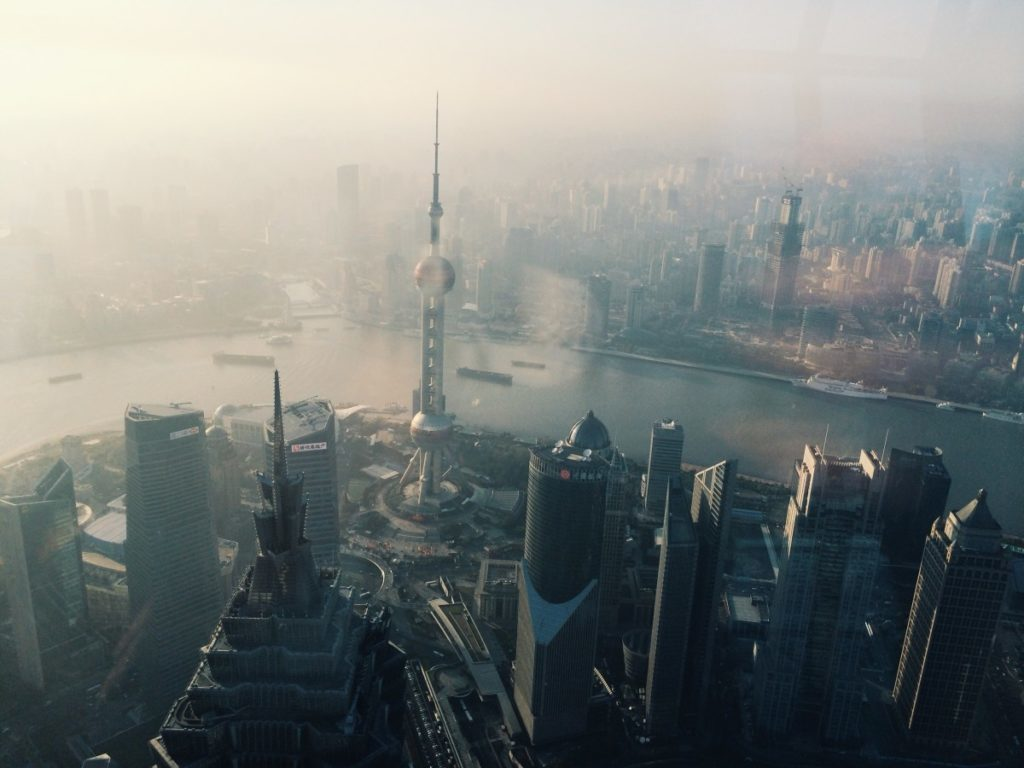
\includegraphics[width=3.67708in,height=\textheight]{images/Shanghai.jpg}

}

\caption{Photo of smog in Shanghai.}

\end{figure}%

Only \textbf{one person in ten} lives in a city that complies with the
World Health Organisation Air quality guidelines.

Fine particular matter was associated with an estimated 2,000 premature
deaths and 22,500 lost life years in Scotland in 2010. There are 38
``Air Quality Management Areas'' (AQMAs) which breach or are likely to
breach legal limits. The Cleaner Air for Scotland strategy seeks to
reduce air pollution across Scotland. It aims to achieve the ``ambitious
vision for Scotland to have the best air quality in Europe''.

There are 99 air quality monitoring stations in Scotland capturing
PM\(_{2.5}\), PM\(_{10}\), NO\(_2\), NO\(_\text{X}\), SO\(_2\) and
O\(_3\).

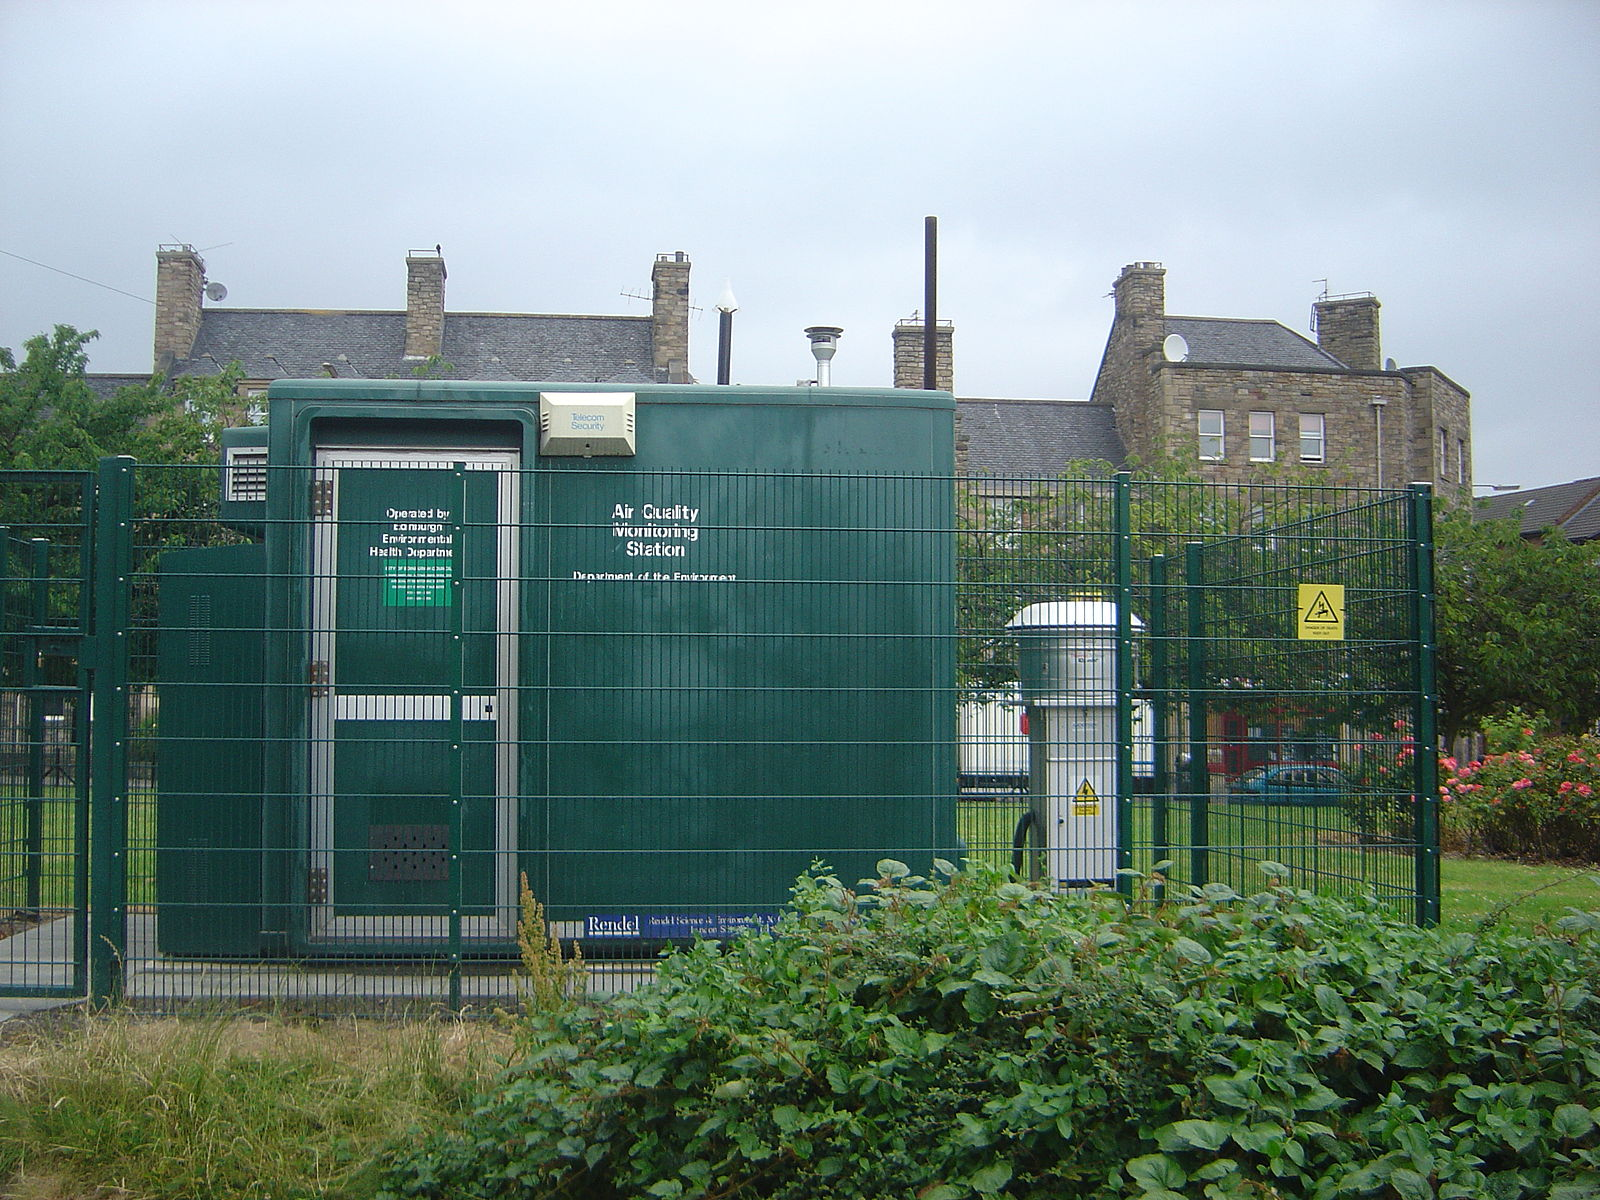
\includegraphics[width=\textwidth,height=2.60417in]{images/EdinburghStation.jpg}
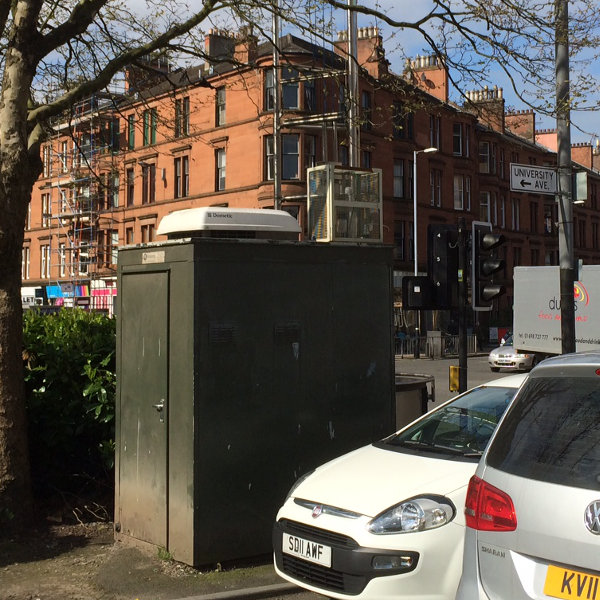
\includegraphics[width=\textwidth,height=2.60417in]{images/GlasgowStation.jpg}

The map below shows the placement of the monitors. Live data are
available at \href{http://www.scottishairquality.scot/}{Scottish Air
Quality}.

\begin{figure}[H]

{\centering 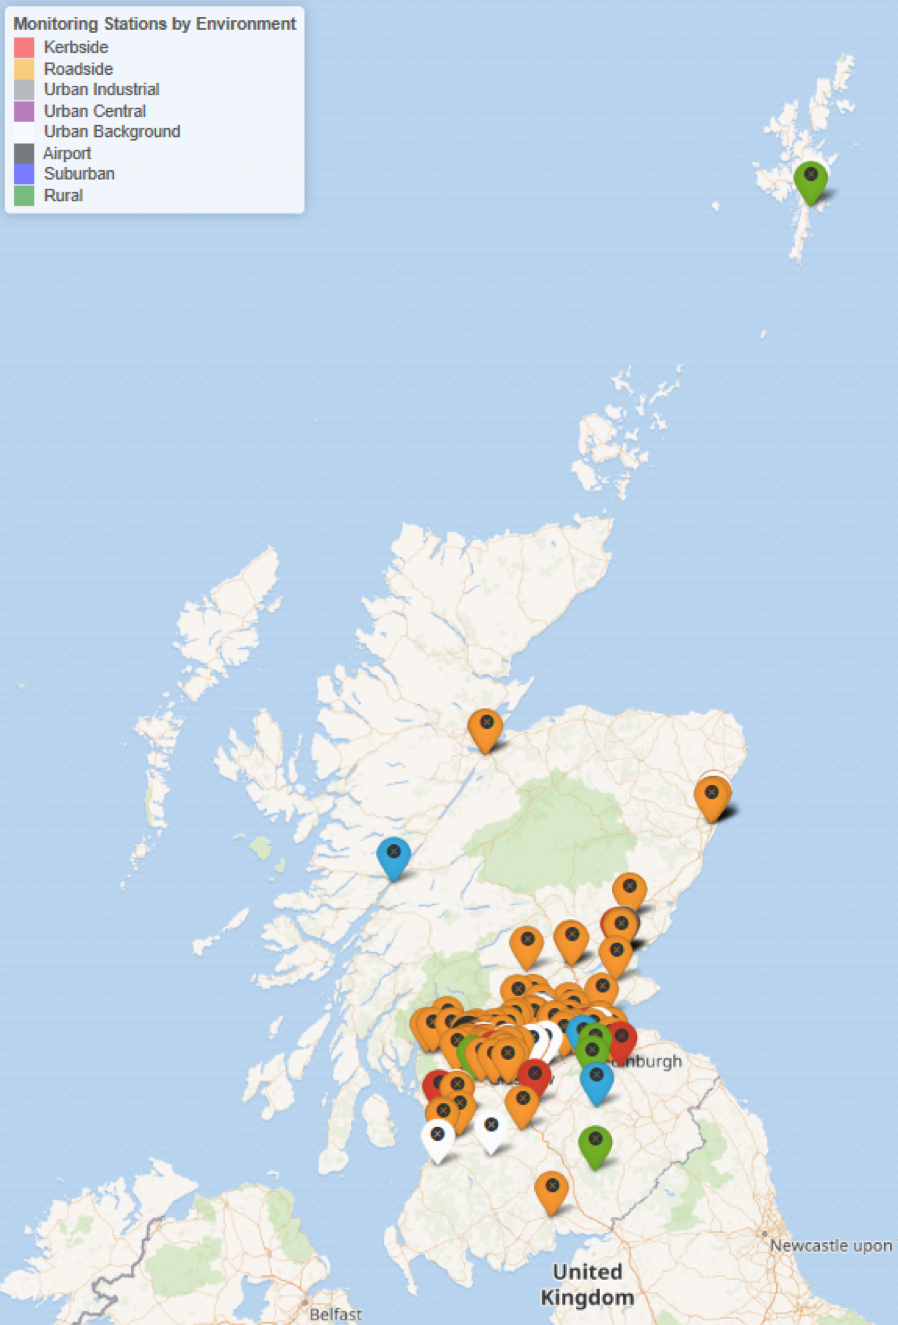
\includegraphics[width=2.875in,height=\textheight]{images/Monitor4.png}

}

\caption{Monitoring station map.}

\end{figure}%

The data from these monitors can be used to estimate the pollution
levels across Scotland.

\begin{figure}[H]

{\centering 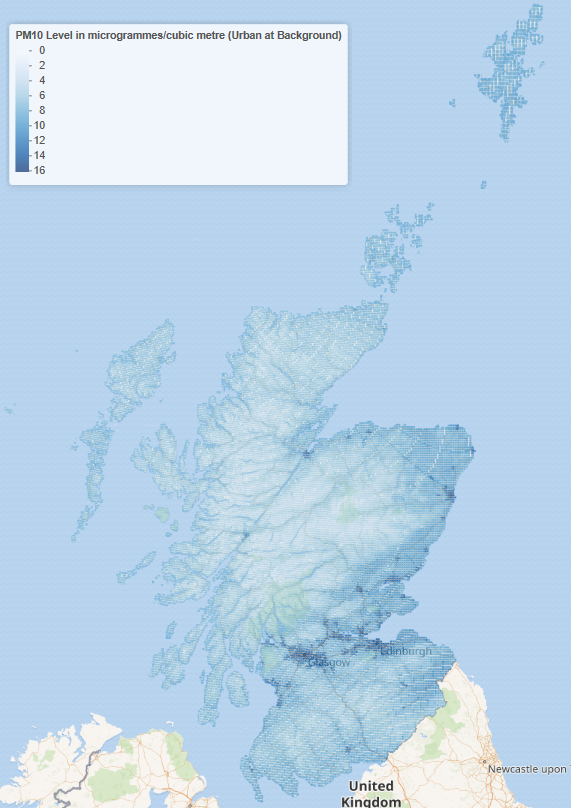
\includegraphics[width=2.8125in,height=\textheight]{images/Result-PM10.png}

}

\caption{Estimated PM\(_{10}\) levels.}

\end{figure}%

\end{tcolorbox}

\begin{tcolorbox}[enhanced jigsaw, breakable, bottomrule=.15mm, toprule=.15mm, colbacktitle=quarto-callout-tip-color!10!white, bottomtitle=1mm, arc=.35mm, opacitybacktitle=0.6, titlerule=0mm, colframe=quarto-callout-tip-color-frame, toptitle=1mm, title={Exercise 4}, rightrule=.15mm, leftrule=.75mm, left=2mm, colback=white, opacityback=0, coltitle=black]

The example above shows a map of estimated PM\(_{10}\) levels across
Scotland. What information do we not have, which we would normally
expect to see here?

Solution

The main thing missing here is the lack of uncertainty information. It
seems that most of the monitoring stations are in the Central Belt of
Scotland (where most of the pollution might be expected), so we'd expect
to see lower uncertainty there than in areas further from a monitoring
station.

We might also like to know more about the temporal aspects of the data.
Is the prediction map for the same time that the data were collected, or
do frequencies of collection vary across the monitoring stations?

Also, are these predictions just from the station data, or do we have
other sources that are combined with these? (For at least some
variables, we might have satellite data available that provide us with
measurements across a fine spatial grid, which we can combine with
monitoring station data through ``data fusion''.) In any case, we'd like
to know how these predictions are made.

You may have thought of some other ideas too. We can discuss these in
the lectures.

\end{tcolorbox}

\section{Quantification}\label{quantification}

Understanding and measuring quantities is a fundamental part of all
science, not just statistics. As scientists, we use data to understand
the process which we are investigating. These data have two main sources
of uncertainty or error:

\begin{itemize}
\tightlist
\item
  \textbf{Inherent variability} of the process itself (the thing we are
  measuring is variable).
\item
  \textbf{Imprecise knowledge} of the process (our measurements may not
  be accurate).
\end{itemize}

The plots below illustrate the trends in several climate change
measures. Both sources of variability will be present, but how much of
each?

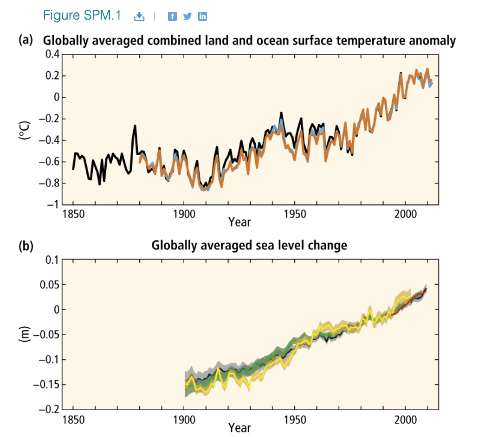
\includegraphics[width=5.20833in,height=\textheight]{images/TempAndSea.png}
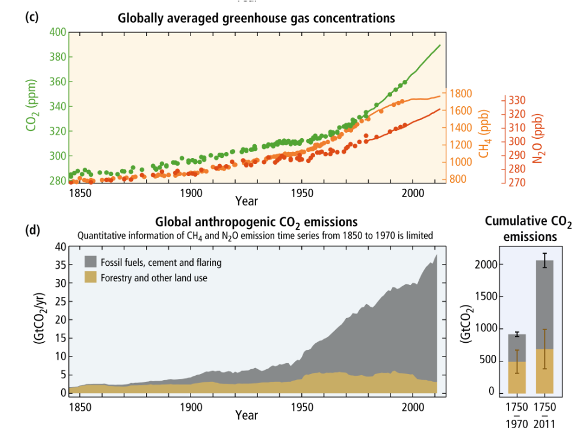
\includegraphics[width=5.20833in,height=\textheight]{images/GreenhouseCO2.png}

A big part of our role as statisticians is to ask questions of both our
data and our models. How were our data collected? Are they
representative of the population? How much uncertainty do we have? Are
our models valid? Are the assumptions reasonable? Does the model make
sensible predictions? How much uncertainty do we have in our results?
These skills are particularly crucial in applied areas such as
environmental and ecological statistics.

\begin{tcolorbox}[enhanced jigsaw, breakable, bottomrule=.15mm, toprule=.15mm, colbacktitle=quarto-callout-important-color!10!white, bottomtitle=1mm, arc=.35mm, opacitybacktitle=0.6, titlerule=0mm, colframe=quarto-callout-important-color-frame, toptitle=1mm, title={Example: Arctic sea ice cover}, rightrule=.15mm, leftrule=.75mm, left=2mm, colback=white, opacityback=0, coltitle=black]

Submarines have been used to measure Arctic sea ice. Over time, the ice
has shrunk both in terms of thickness and extent. We may soon see
ice-free summers, which will have a devastating impact on sea life.

\begin{figure}[H]

{\centering 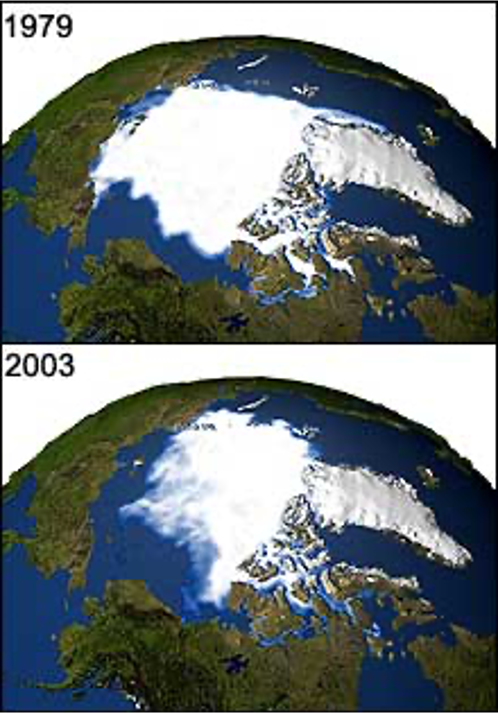
\includegraphics[width=2.08333in,height=\textheight]{images/ArcticIceMap.png}

}

\caption{Arctic ice coverage in 1979 and 2003.}

\end{figure}%

This
\href{https://interactive.carbonbrief.org/when-will-the-arctic-see-its-first-ice-free-summer/}{interactive
map} provides an illustration of the changes.

\end{tcolorbox}

\begin{tcolorbox}[enhanced jigsaw, breakable, bottomrule=.15mm, toprule=.15mm, colbacktitle=quarto-callout-tip-color!10!white, bottomtitle=1mm, arc=.35mm, opacitybacktitle=0.6, titlerule=0mm, colframe=quarto-callout-tip-color-frame, toptitle=1mm, title={Exercise 5}, rightrule=.15mm, leftrule=.75mm, left=2mm, colback=white, opacityback=0, coltitle=black]

How might we quantify the trend in Arctic sea ice cover, and what
problems might we encounter in aiming to do this?

Solution

We might want to present this as a graph of total estimated sea ice
cover over time, across many years. Some problems with this approach
could be data availability over time (satellites or submarines not
covering the whole area, or only at certain timepoints, and lack of data
in earlier years), and the difficulty in estimating coverage at any
timepoint from these measurements --- statistical approaches would be
vital to estimate this and the associated uncertainty.

Note that the use of before and after images (like in the above example)
might not be thought of as the best idea in statistics (since they could
be misused, with particular years cherry-picked to back up an incorrect
claim), but such images can be useful in illustrating a trend to the
general public, as long as this is also presented with additional
complete information about the general patterns.

\end{tcolorbox}

\section{Understanding our data:
trends}\label{understanding-our-data-trends}

Much of the statistical analysis of environmental and ecological data
will focus on identifying \textbf{trends}. The statistical definition of
a trend is \emph{a long-term change in the mean level}. Trends aren't
restricted to being linear, and we will also look at examples of
non-linear trends, and changepoints.

Trends generally tend to focus on the \textbf{mean} of the data.
However, we may also be interested in observing other aspects of the
statistical distribution. \textbf{Extreme value theory} looks
specifically at the limits of our distribution, and focuses on rare (or
extreme) events.

We'll cover this more later in the course.

\section{Policy and legislation}\label{policy-and-legislation}

A great deal of environmental statistical research is funded by
governments and regulatory bodies. They need to know where the biggest
challenges lie so that they can allocate their resources appropriately.
Evidence-based policy relies on measuring changes and also evaluating
the impacts of existing policies. However, the environment will be one
of many competing policy areas, and every government will prioritise it
differently.

\begin{tcolorbox}[enhanced jigsaw, breakable, bottomrule=.15mm, toprule=.15mm, colbacktitle=quarto-callout-important-color!10!white, bottomtitle=1mm, arc=.35mm, opacitybacktitle=0.6, titlerule=0mm, colframe=quarto-callout-important-color-frame, toptitle=1mm, title={Example of international cooperation and negotiations: COP}, rightrule=.15mm, leftrule=.75mm, left=2mm, colback=white, opacityback=0, coltitle=black]

\begin{figure}[H]

{\centering 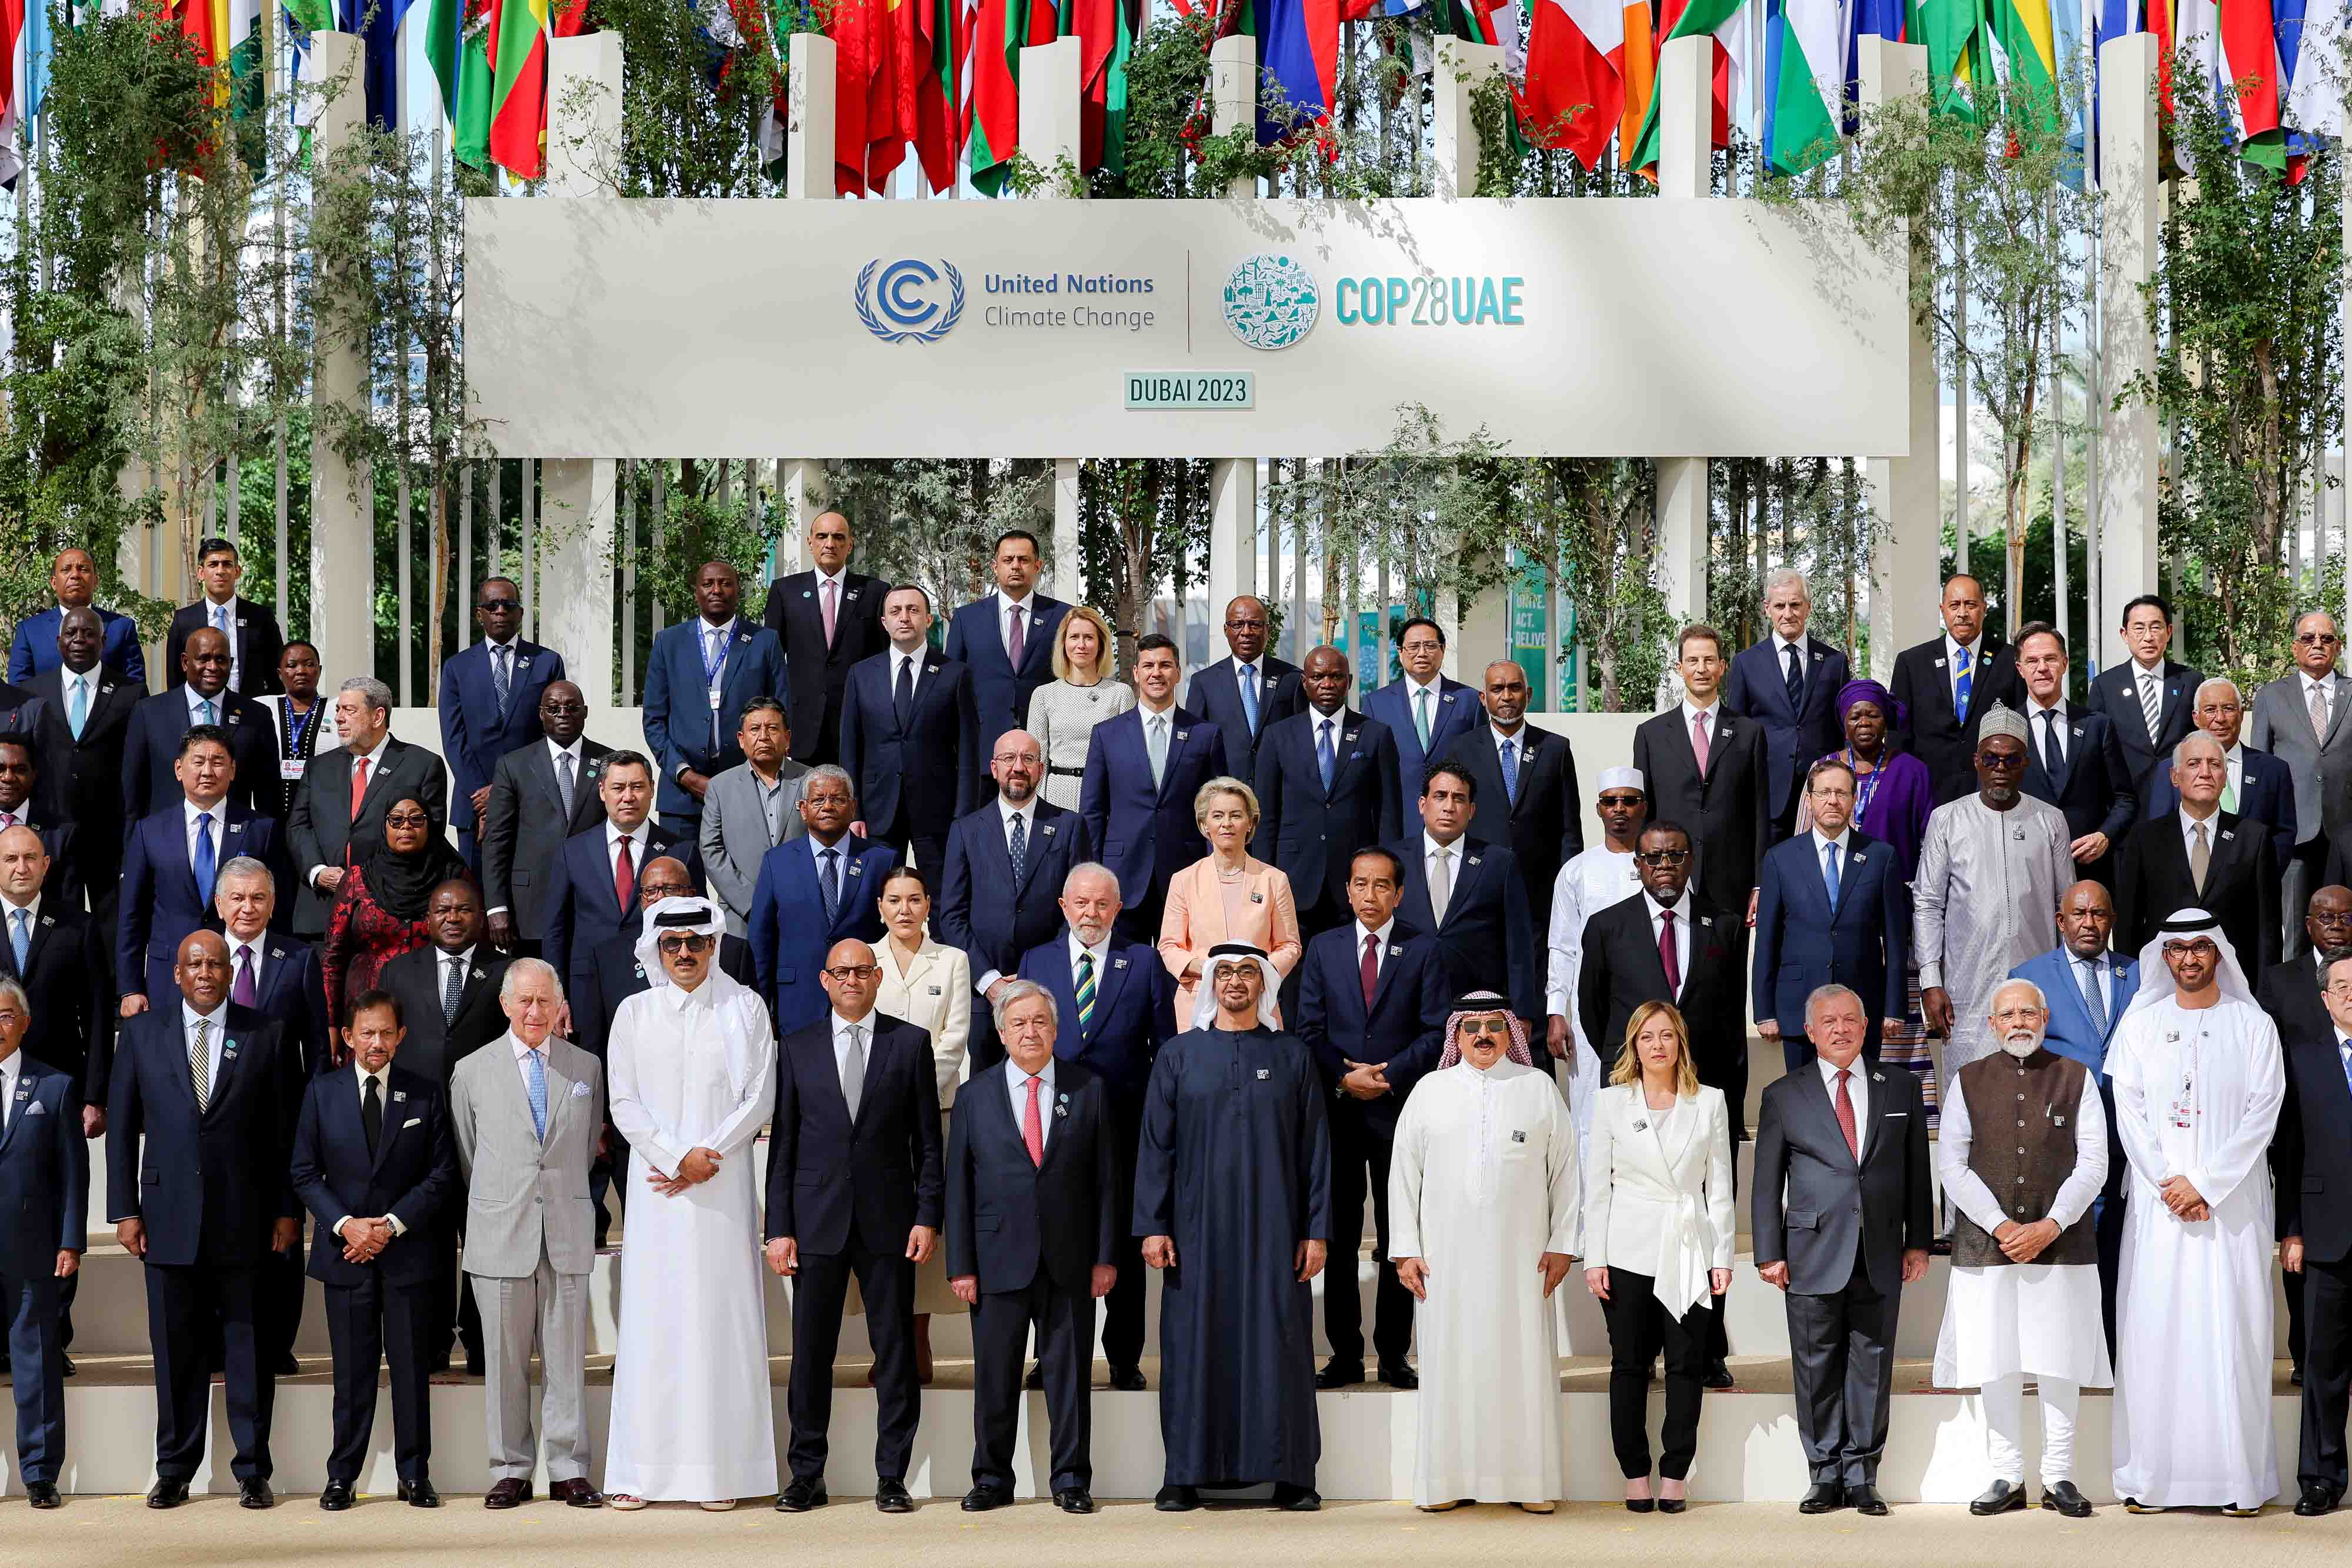
\includegraphics[width=5.20833in,height=\textheight]{images/COP28.jpg}

}

\caption{Team photograph from COP28 in 2023.}

\end{figure}%

COP is the United Nations Climate Change Conference that takes place
annually (\href{https://www.un.org/en/climatechange/cop26}{held in
Glasgow in 2021}), where most countries' governments come together to
try to agree on goals to limit global temperature rise and achieve net
zero emissions. The most recent conference was
\href{https://unfccc.int/cop29/about-cop29}{COP29}, which took place in
Baku, Azerbaijan, in November 2024.

One of the key achievements of COP29 was an agreement by wealthier
countries to pay at least US \$300 billion per year to less wealthy
countries to help finance their mitigation of climate change impacts,
and to transform their economies away from fossil fuels. However, there
was limited progress in other sectors.

A report on COP29 and its implications for the UK is available from the
UK's Climate Change Committee
\href{https://www.theccc.org.uk/publication/cop29-key-outcomes-and-next-steps-for-the-uk/}{here}.

\end{tcolorbox}

Environmental policy tends to use very specific language:
\emph{objectives, targets, guide values, standards, reductions relative
to a baseline}. Policy often prescribes monitoring quantities of
interest over space and/or time. Quantities of interest include
\emph{water, air and noise pollution, waste management, radioactive
substances, biodiversity and animal and plant species}.

Legislation is the legal framework used to implement policy. Most
legislation focuses on setting targets or safe levels for the
pollutants. A number of regulatory bodies exist specifically to monitor
such things,
e.g.~\href{https://beta.sepa.scot/about-sepa/who-we-are/}{Scottish
Environment Protection Agency} (SEPA, for Scotland), the
\href{https://www.gov.uk/government/organisations/environment-agency/about}{Environment
Agency} (EA, for England) and the
\href{https://www.eea.europa.eu/en}{European Environment Agency} (EEA,
for the EU). As well as regulatory bodies, the
\href{https://www.theccc.org.uk/about/}{Climate Change Committee}
advises governments within the UK on reducing emissions and addressing
climate change impacts.

Much of our data come from \emph{routine monitoring} of our
environmental quantities of interest. Government agencies often make
these data available to researchers and/or the public. These data are
used to assess compliance with legislation as well as to identify
environmental trends and their potential impacts on society.

\begin{tcolorbox}[enhanced jigsaw, breakable, bottomrule=.15mm, toprule=.15mm, colbacktitle=quarto-callout-note-color!10!white, bottomtitle=1mm, arc=.35mm, opacitybacktitle=0.6, titlerule=0mm, colframe=quarto-callout-note-color-frame, toptitle=1mm, title={Example of Natural Capital and Ecosystem Assessment (NCEA) programme}, rightrule=.15mm, leftrule=.75mm, left=2mm, colback=white, opacityback=0, coltitle=black]

The UK Government's Natural Capital and Ecosystem Assessment (NCEA)
programme aims to provide a comprehensive understanding of the state of
the natural environment to inform better decision-making for its
protection and enhancement. By integrating data collection, mapping,
standardized protocols, and detailed reporting, the NCEA seeks to halt
biodiversity loss, support climate adaptation and mitigation, and ensure
sustainable management of natural capital for future generations. This
evidence-based approach helps identify environmental trends, risks, and
opportunities to guide policy and conservation efforts.

The brochure below provides an overview of some of the key resources
produced by the NCEA.

\end{tcolorbox}

\begin{tcolorbox}[enhanced jigsaw, breakable, bottomrule=.15mm, toprule=.15mm, colbacktitle=quarto-callout-tip-color!10!white, bottomtitle=1mm, arc=.35mm, opacitybacktitle=0.6, titlerule=0mm, colframe=quarto-callout-tip-color-frame, toptitle=1mm, title={Exercise 6}, rightrule=.15mm, leftrule=.75mm, left=2mm, colback=white, opacityback=0, coltitle=black]

Download the NCEA. brochure and read to three case studies and identify
(1) the problem that is being address (2) the proposed solution and its
(3) policy impact. Then, think about how would you present the data.

\end{tcolorbox}

\section*{References}\label{references}
\addcontentsline{toc}{section}{References}

Some general reference books that you may find useful include the
following:

\begin{itemize}
\tightlist
\item
  Piegorsch, W. W., \& Bailer, A. J. (2005). \emph{Analyzing
  environmental data}. Wiley. (Available from the University Library as
  an e-book \href{https://go.exlibris.link/6wbh6zq0}{here}.)
\item
  Barnett, V. (2004). \emph{Environmental statistics: Methods and
  applications}. Wiley. (Available from the University Library as an
  e-book \href{https://go.exlibris.link/TbMBCTkV}{here}.)
\item
  Manly, B. F. J. (2001). \emph{Statistics for environmental science and
  management}. Chapman \& Hall/CRC. (No e-book available, but
  \href{https://go.exlibris.link/Jcyj94mj}{a physical copy is available
  from the University Library}.)
\end{itemize}



\end{document}
